\PassOptionsToPackage{hyphens}{url}
\documentclass[11pt,a4paper]{article}
\usepackage[T1]{fontenc}
\usepackage[utf8]{inputenc}
\usepackage[spanish,es-noquoting,es-tabla]{babel}
\usepackage{amsmath,amssymb}
\usepackage{booktabs}
\usepackage{graphicx}
\usepackage[margin=2.4cm]{geometry}
\usepackage{microtype}
\usepackage[colorlinks=true,linkcolor=black,urlcolor=blue,citecolor=black]{hyperref}
\usepackage{xcolor}
\urlstyle{tt}
\usepackage{enumitem}
\usepackage{tocloft}
\usepackage{listings}
\setlength{\cftsecnumwidth}{2.4em}
\setlength{\cftsubsecnumwidth}{3.2em}
\setlist{nosep}
\lstset{basicstyle=\ttfamily\footnotesize,columns=fullflexible,frame=single,
        framerule=0.3pt,rulecolor=\color{gray},xleftmargin=1em,xrightmargin=1em}

\newcommand{\dd}{\mathrm{d}}
\newcommand{\etq}[1]{\textcolor{gray}{\texttt{[#1]}}}
\newcommand{\archivo}[1]{\nolinkurl{#1}}
\makeatletter\g@addto@macro{\UrlBreaks}{\do\_\do\-\do\.}\makeatother
\newcommand{\propio}{\textsuperscript{\textcolor{gray}{\,\S}}}
\newcommand{\PuertaFinal}{8/8}
\newcommand{\FaseDosRegresion}{6/6}
\graphicspath{{../salidas/figuras/}}

\title{Superficie libre deformable en SPECTER:\\
implementación lineal, verificación y lo que encontró la puerta}
\author{Lucía Mazaira\\ \small INFINA, CONICET--UBA}
\date{\small Informe de implementación --- 28 de septiembre de 2026}

\begin{document}
\maketitle

\begin{abstract}
\noindent
Se implementó en SPECTER una superficie libre \emph{deformable}, linealizada: el dominio
no se mueve, la cinemática y el balance de tensiones de la superficie se aplican en
$z=L_z$, y la elevación $\eta(x,y,t)$ se integra como un campo 2D propio. El volumen sigue
siendo Navier--Stokes completo. La presión pasa a ser Dirichlet en la superficie, lo que
pidió una rama nueva de \texttt{laplace\_z} y una proyección con una condición distinta en
cada cara; la tensión tangencial deja de ser una condición sobre la vorticidad y se
acopla a la velocidad de la superficie, y ese acople se resuelve \emph{exactamente} con
dos pasadas, porque toda la cadena es lineal y diagonal en los modos horizontales. La
puerta de aceptación se escribió antes, en rojo, sin fórmula analítica del resultado:
compara la trayectoria $\eta(t)$ contra una referencia de diferencias finitas propia que
se verifica a sí misma por balance de energía. La primera versión dio \textbf{7/8}: el
chequeo de orden temporal falló (1{,}45 en vez de 2), y la búsqueda de la causa encontró
un defecto que \emph{ya estaba en el camino free-slip plano de la Fase 2}: una pérdida de
energía por paso que no depende de $dt$. Corregido en los dos caminos, la puerta da
\textbf{\PuertaFinal}, la de la Fase~2 sigue en 6/6, y las tasas de la Fase~4 vueltas a
medir no se mueven ($\le5\cdot10^{-10}$). Se muestra además que el modo vortical del experimento
---horizontal, sin $w$--- no siente la deformación a orden lineal: su efecto sobre
$\alpha$ es puramente no lineal, $O(\mathrm{Fr}^2)$.
\end{abstract}

\noindent\small Convención: un \propio{} marca una derivación, estimación o hipótesis
hecha en esta sesión y no validada contra bibliografía. Las etiquetas \etq{D-nn},
\etq{H-nn}, \etq{V-nn} remiten a \archivo{DECISIONES.md}.\normalsize

\tableofcontents

%=====================================================================
\section{Qué se pidió y en qué estado estaba}

El pedido de Lucía (2026-09-28) fue revisar qué había dejado sin hacer una sesión
anterior (de otro agente, codex) y seguir con la superficie libre, \emph{``with
deformations this time''}. Hasta acá SPECTER tenía una superficie \emph{free-slip plana}
\etq{V-09}: $w=0$ y tensión tangencial nula en $z=L_z$. La deformación estaba fuera de
alcance por \etq{D-28}, que estimaba $\eta/h\sim10^{-5}$ en la celda.

\paragraph{Lo que había dejado la sesión anterior.} Un directorio no versionado,
\archivo{research/2026-09-25_nonlinear_free_surface/}, con una derivación de una
jerarquía cúbica en amplitud, núcleos de frontera en Python y en Fortran autónomo, una
referencia 2D viscosa pequeña (no SPECTER), una referencia inviscida de ondas y una revisión
independiente. Se volvieron a correr sus siete chequeos: pasan todos (pico de memoria
150\,MB). Lo que \emph{no} había hecho:
\begin{itemize}
\item nada de SPECTER había cambiado (el árbol de trabajo coincidía byte a byte con el
  parche de la Fase 2);
\item el \archivo{report.pdf} que anunciaba su README no existía;
\item \archivo{ESTADO.md} y \archivo{DECISIONES.md} se habían quedado en el 2026-09-23 y no
  mencionaban nada de ese trabajo; no había ningún commit.
\end{itemize}
Además, su jerarquía cúbica suponía que existía una superficie deformable \emph{lineal}
en otra sesión en Sakura, que nunca estuvo en el repositorio. Como su esquema cúbico
resuelve el mismo problema lineal una vez por orden, la lineal es un requisito previo.
Lucía eligió explícitamente implementar primero la lineal en SPECTER \etq{D-49}.

%=====================================================================
\section{El modelo}

\subsection{Las condiciones de una superficie libre viscosa}

Para una interfaz $z=h+\eta(x,y,t)$ entre el fluido y una atmósfera de presión constante
$p_e$, Wang, Tice y Kim escriben, en su §1.1 \cite{wtk2014},
\begin{equation}
(\bar p\,I-\mu\,\mathbb{D}v)\,n = p_e\,n-\sigma H\,n,\qquad
n=\frac{(-\partial_1\eta,-\partial_2\eta,1)}{\sqrt{1+|\nabla_*\eta|^2}},\qquad
H=\nabla_*\cdot\frac{\nabla_*\eta}{\sqrt{1+|\nabla_*\eta|^2}},
\tag{WTK 1.4--1.6}
\end{equation}
con $(\mathbb{D}v)_{ij}=\partial_jv_i+\partial_iv_j$ y la normal hacia arriba, y la
condición cinemática $\partial_t\eta=v_3-v_1\partial_1\eta-v_2\partial_2\eta$ (WTK 1.8).
La gravedad es una fuerza de volumen $-g\rho e_3$ (WTK 1.3). Esas ecuaciones se leyeron en
el original (arXiv:1109.1798v2) y su DOI se resolvió contra Crossref. Son las ecuaciones
\emph{no lineales}; la forma linealizada que el paper escribe (1.25) no tiene tensión
superficial, así que la linealización con capilaridad de abajo es de esta sesión.

\subsection{La linealización que usa SPECTER\propio}

SPECTER integra la presión cinemática sin la parte hidrostática. Escribiendo
$\bar p=p_e+\rho g(h-z)+\rho p$, la presión total en la superficie es
$p_e-\rho g\eta+\rho p$. A primer orden en la amplitud, evaluando en $z=h$ y con
$\gamma=\sigma/\rho$, la componente normal de (WTK 1.4), sus dos componentes tangenciales
y la cinemática dan
\begin{equation}
\partial_t\eta=w,\qquad
\partial_zu+\partial_xw=0,\quad \partial_zv+\partial_yw=0,\qquad
p=g\,\eta-\gamma\,\nabla_h^2\eta+2\nu\,\partial_zw
\qquad\text{en } z=L_z .
\label{eq:modelo}
\end{equation}
Los dos términos restituyen: para un modo $e^{i\mathbf k\cdot\mathbf x}$ la presión es
$(g+\gamma k^2)\eta+2\nu\partial_zw$. La gravedad \emph{no} entra como fuerza de volumen.
El fondo sigue siendo no-deslizante (o free-slip). El dominio no se mueve y el volumen es
Navier--Stokes completo: es el modelo de «frontera lineal, volumen no lineal». No
representa la geometría no lineal de la superficie; para eso está la jerarquía cúbica de
la sesión anterior o una formulación ALE (§\ref{sec:falta}).

\subsection{Qué modos mueve la superficie\propio}
\label{sec:toroidal}

Un modo horizontal $\mathbf k$ se separa en una parte \emph{toroidal} (velocidad horizontal
perpendicular a $\mathbf k$, sin $w$ y sin presión) y una \emph{poloidal} (velocidad en el
plano de $\mathbf k$ y $z$). Con $w\equiv0$ y $p\equiv0$ las tres condiciones
\eqref{eq:modelo} se reducen a las de la superficie plana, así que \textbf{a orden lineal la
parte toroidal no siente la deformación}: decae exactamente con
$\nu[(\pi/2h)^2+k^2]=\alpha(1+4\varepsilon^2/\pi^2)$, la tasa de la Fase~1 \etq{V-07}. El
flujo cuasi-2D del experimento es esencialmente toroidal. La superficie entra sólo en la
parte poloidal, que son ondas de gravedad-capilaridad amortiguadas (§\ref{sec:celda}). El
acople entre las dos es no lineal: la presión dinámica $\rho U^2$ levanta la superficie
$\eta\sim U^2/g$, que es exactamente la estimación de \etq{D-28}. El desacople se comprueba en
SPECTER en §\ref{sec:extras} (E1 y E1b), bit a bit.

\textbf{Lo que esta implementación no puede calcular.} Al orden en que la deformación sí
cambia $\alpha$, $O(\mathrm{Fr}^2)$, entran también los términos de transferencia
$\eta\,\partial_z(\cdot)$ ---evaluar las condiciones en $h+\eta$ y no en $h$, es decir, el
cambio de espesor---, que un modelo lineal en la frontera descarta por diseño. Lo señaló el
verificador independiente y se acepta: comparar \texttt{freesurface} contra \texttt{freeslip}
mediría sólo la parte del efecto que pasa por el flujo poloidal inducido. El efecto completo
pide el orden cuadrático de la jerarquía de la sesión anterior.

%=====================================================================
\section{Cómo lo impone SPECTER}

\subsection{El esquema en el que hay que encajarlo}

En cada subpaso $o=\texttt{ord},\dots,1$ del Runge--Kutta, SPECTER avanza un campo sin
presión, le impone condiciones de contorno y proyecta \cite{fontana2020}:
\[
v^*=v^n+\tfrac{dt}{o}\,F(v^{(o+1)}),\qquad v^{(o)}=v^*-\nabla d .
\]
La variable \texttt{pr} guarda $d=(dt/o)\,p$ del subpaso en que se calculó: se deduce de
que \texttt{noslip\_z} reescala el \texttt{pr} del subpaso anterior por $(o+1)/o$ y de que
la salida lo divide por $dt$ (no está en el paper; el código lo marca como
\texttt{!TODO update documentation about p' = dt*p}).

\subsection{(a) La presión: Dirichlet arriba}

La tensión normal \emph{prescribe} $p$ en la superficie, así que $d$ es Dirichlet en
$z=L_z$, con el dato
\begin{equation}
d(L_z)=\frac{dt}{o}\Big[(g+\gamma k^2)\,\eta^{(o+1)}+2\nu\,\partial_zw^{(o+1)}\Big],
\label{eq:dirichlet}
\end{equation}
evaluado en el estado del subpaso anterior, como cualquier otro término del miembro
derecho de un Runge--Kutta explícito. En el fondo sigue la condición de Neumann que deja
$w=0$ después de proyectar. Hicieron falta dos cosas nuevas:
\begin{itemize}
\item \textbf{la rama Neumann($z=0$)--Dirichlet($z=L_z$) de \texttt{laplace\_z}}, la
  \emph{opuesta} a la que se agregó en la Fase~2 \etq{H-08}. En la base del archivo,
  $\phi=C_1e^{k(z-L_z)}+C_2e^{-kz}$ con $r=e^{-kL_z}$ y datos $g_0=\phi'(0)$,
  $g_1=\phi(L_z)$:
  \[
  C_1=\frac{g_1+r\,g_0/k}{1+r^2},\qquad C_2=\frac{r\,g_1-g_0/k}{1+r^2},\qquad
  \phi_{k=0}=g_0z+(g_1-g_0L_z).
  \]
  Mismo denominador $1+r^2$ que la rama espejo: no tiene resonancia.
\item \textbf{\texttt{sol\_project\_fs}}: \texttt{sol\_project} tiene un único
  \texttt{bctarget} para las dos caras, y acá hacen falta distintos (Neumann abajo,
  Dirichlet inhomogéneo arriba). La rutina nueva es la misma proyección con la condición
  de cada cara explícita; el camino plano no se tocó.
\end{itemize}

\subsection{(b) La elevación}

$\eta^{(o)}=\eta^n+(dt/o)\,w^{(o+1)}(L_z)$: el mismo esquema que la velocidad. $\eta$ vive
en el espacio $(k_y,k_x)$, con la misma normalización que un campo en $(z,k_y,k_x)$, y el
modo medio se conserva (es $\int w\,\dd A$ en la superficie, que la incompresibilidad
anula).

\subsection{(c) La tensión tangencial y su acople exacto}

La tensión tangencial es vorticidad más un término de $w$:
$\tau_x=\partial_zu+ik_xw=\omega_y+2ik_xw$, con $\omega_y=\partial_zu-ik_xw$. La
vorticidad no cambia al proyectar (el rotor de un gradiente es cero), así que pedir
$\tau_x=0$ sobre el campo \emph{proyectado} es, sobre $v^*$,
\begin{equation}
\partial_zv^*_x=ik_x\,(v^*_z-2W),\qquad \partial_zv^*_y=ik_y\,(v^*_z-2W),
\label{eq:tension}
\end{equation}
con $W=w(L_z)$ \emph{después} de proyectar. Con $W=0$ es exactamente \texttt{freeslip\_z}
de la Fase~2. Pero $W$ no se conoce antes de proyectar: es el problema que
\archivo{teoria/superficie_libre_v_estrella_y_p.md} §4.4 dejaba abierto (iterar o
rezagar).

\paragraph{La salida exacta\propio.} Toda la cadena ---reconstrucción de Neumann,
continuación FC-Gram, proyección--- es lineal y está desacoplada por modo horizontal. Para
cada modo, entonces, $W_{\text{final}}=A_{\mathbf k}+B_{\mathbf k}W$, con $B_{\mathbf k}$
fijo para toda la corrida (depende de la malla y de $k$, no del estado ni de $dt$). Se
calcula una sola vez al arrancar, pasando la cadena sobre un campo nulo con $W=1$ en todos
los modos. En cada subpaso:
\begin{enumerate}
\item una pasada con un $W$ de prueba $W_g$ (el del subpaso anterior) da
  $W_1=A_{\mathbf k}+B_{\mathbf k}W_g$;
\item $W^\star=(W_1-B_{\mathbf k}W_g)/(1-B_{\mathbf k})$ es el punto fijo exacto;
\item se restauran los campos guardados y una segunda pasada impone $W^\star$.
\end{enumerate}
El diagnóstico mide cuánto difiere el $W$ que sale del impuesto: $5{,}6\cdot10^{-16}$
relativo, redondeo. En la malla de la puerta $\max|B_{\mathbf k}|=9{,}6\cdot10^{-4}$. El
parámetro \texttt{fscoup=1} hace una sola pasada con el $W$ rezagado: tiene error $O(dt)$ en
la tensión y existe sólo como control negativo de la puerta.

\subsection{(d) El defecto que encontró la puerta}
\label{sec:defecto}

La primera versión pasó siete de los ocho chequeos. Falló F6: el orden temporal observado
en el caso A, con \texttt{ORD=2}, fue \textbf{1{,}45}, con diferencias sucesivas
$1{,}47\cdot10^{-7}$ y $5{,}39\cdot10^{-8}$. Como la puerta no se edita, se buscó la causa.
La secuencia de controles, en orden:

\begin{enumerate}
\item \textbf{No es el fondo no-deslizante}: con fondo free-slip el orden es 1{,}48.
\item \textbf{No es el esquema de SPECTER en general}: los caminos \texttt{freeslip} y
  \texttt{noslip} planos, sobre un modo 3D con $w\neq0$, dan orden $\approx2{,}4$ en la
  energía.
\item \textbf{No es el acople de $\eta$}: partiendo de un modo de velocidad suave, la
  superficie deformable da orden $\approx3$ con $g=0$ y con $g=1$.
\item \textbf{No es la condición inicial incompatible}. Arrancar del reposo con
  $\eta\neq0$ viola la compatibilidad (en $t=0^+$, $\partial_tu=-\nabla p_0$ no respeta
  el no-deslizamiento ni la tensión nula) y se esperaba una reducción de orden por las
  capas límite impulsivas. Pero el mismo RK2 aplicado a la referencia MAC, con la misma
  condición inicial y el mismo $\Delta z$, da orden \textbf{2{,}00} exacto. La hipótesis
  quedó refutada.
\item \textbf{Es un error por paso.} La diferencia entre SPECTER y el RK2 de la referencia
  (extrapolada en el espacio) debería ser independiente de $dt$ si SPECTER fuera un RK2
  consistente de alguna discretización espacial. No lo es: crece al achicar $dt$
  ($8{,}07$, $8{,}29$, $8{,}61$, $9{,}20\cdot10^{-7}$ para
  $dt=10^{-3}\dots1{,}25\cdot10^{-4}$), aproximadamente en proporción al número de pasos.
  Con $N_z=64$ domina todo: las diferencias sucesivas se \emph{duplican} al dividir $dt$
  por dos.
\item \textbf{Aislado con $dt\to0$}: con $dt=10^{-9}$ y $10^{-10}$ el miembro derecho es
  nulo y el estado no debería cambiar. En los caminos \texttt{freeslip} y
  \texttt{freesurface} la energía de \archivo{balance.txt} cambia $-1{,}4\cdot10^{-7}$ por
  paso con $N_z=64$ y $\approx-10^{-8}$ con $N_z=128$, \emph{igual} para los dos $dt$; en
  \texttt{noslip} el cambio es proporcional a $dt$, el físico.
\end{enumerate}

\paragraph{La causa.} Los caminos \texttt{freeslip} y \texttt{freesurface} necesitan
$v^*_z$ en la cara, y el parche de la Fase~2 lo conseguía mandando $v_z$ por
\texttt{goto\_domain\_w\_boundaries} y de vuelta por \texttt{goto\_3d\_fourier}. Esa vuelta
\emph{recalcula la continuación FC-Gram} de $v_z$ a partir de sus valores físicos, y después
de una proyección ---que actúa sobre todo el dominio periódico extendido--- la
continuación de $v_z$ ya no coincide con la que FC-Gram le daría a sus valores físicos. Cada
subpaso cambia entonces el campo en una cantidad que \emph{no se anula con $dt$}. El camino
\texttt{noslip} nunca transforma $v_z$, y por eso no lo tiene. Un primer intento de
corrección, suponiendo que el defecto era de la reconstrucción de Neumann del valor de
borde, no cambió nada y se descartó.

\paragraph{La corrección.} $v^*_z$ se queda en el dominio $(k_z,k_y,k_x)$ y sólo se leen sus
trazas en las caras (\texttt{fs\_trace}). Con eso el cambio por paso a $dt\to0$ pasa a ser
proporcional a $dt$ ($-2{,}2\cdot10^{-9}$ y $-2{,}2\cdot10^{-10}$ con $N_z=128$), y el orden
del caso A es \textbf{2{,}00}, con diferencias $1{,}381\cdot10^{-7}$ y
$3{,}450\cdot10^{-8}$, a 6\,\% del RK2 puro de la referencia ($1{,}458\cdot10^{-7}$ y
$3{,}646\cdot10^{-8}$).

\paragraph{Lo que implica para la Fase 2\propio.} El camino \texttt{freeslip\_z} plano, que
ya se usó en las corridas del barrido en $\delta$ y del puente de banda ancha, \emph{tiene
el mismo defecto}. La puerta de la Fase~2 no podía verlo: sus chequeos de tasa (V4, V5)
usan el modo de corte sin estructura horizontal, que no lo tiene (el modo $k=0$ de $v_z$ es
nulo), y V3 mide la tensión, no la energía. Su tamaño depende de la resolución vertical y del
flujo: para el modo de prueba ($k_x=1$) es $\sim10^{-8}$ de la energía por paso con
$N_z=128$ y $\sim1{,}4\cdot10^{-7}$ con $N_z=64$, que es la malla de
\archivo{decaimiento_banda_ancha.py}. Esos números son de la energía de
\archivo{balance.txt}, que \texttt{energy()} suma sólo sobre los puntos \emph{físicos}
(\archivo{pseudospec_hd.f90}, lazos \texttt{k = 1,nz-Cz}): \textbf{es disipación espuria en
el dominio físico}. Una primera versión de este informe decía lo contrario, que era la energía
del dominio extendido; lo refutó el verificador leyendo esa rutina y se comprobó. Sesga las
tasas hacia arriba, y \etq{P-02} es justamente una comparación de tasas.

\textbf{Cuánto afecta a la Fase~4 no se midió.} Una estimación de esta sesión, sin validar:
la deriva por unidad de tiempo es $\delta/dt$, con $\delta$ el cambio por paso. Con
$\delta=1{,}4\cdot10^{-7}$ y $dt=5\cdot10^{-4}$ serían $2{,}8\cdot10^{-4}$ por unidad de
tiempo del código, contra una tasa de energía $2\alpha\approx0{,}2$ en esas unidades: un
$0{,}1$\,\% para el modo de prueba, que tiene $w\neq0$. Las corridas de la Fase~4 arrancan
con $w=0$ (flujo horizontal cuasi-2D), donde el mecanismo sólo actúa a través del $v_z$ que
genera la no linealidad, así que el sesgo ahí debería ser menor. Es una estimación, no una
medida.
\paragraph{Corregido también en el camino plano \etq{D-50}.} Lucía decidió corregir
\texttt{freeslip\_z}: recibe la traza de $v^*_z$ en la cara (\texttt{trace\_z}) y $v_z$ ya no
hace la vuelta. Antes y después, con el mismo modo de prueba:

\begin{center}\footnotesize
\begin{tabular}{lccc}
\toprule
 & \multicolumn{2}{c}{deriva por paso, $dt=10^{-9}$ / $10^{-10}$} & $N_z=64$: diferencias \\
 & $N_z=64$ & $N_z=128$ & entre $dt$ sucesivos\\
\midrule
antes & $-1{,}44$ / $-1{,}43\cdot10^{-7}$ & $-1{,}05\cdot10^{-8}$ / $-8{,}4\cdot10^{-9}$ & $2{,}5\to3{,}9\to6{,}7\cdot10^{-6}$\\
después & $-9{,}4\cdot10^{-10}$ / $-8{,}0\cdot10^{-11}$ & $-2{,}25\cdot10^{-9}$ / $-2{,}25\cdot10^{-10}$ & $9{,}6\to7{,}1\to4{,}2\cdot10^{-7}$\\
\bottomrule
\end{tabular}
\end{center}

Después de la corrección la deriva es proporcional a $dt$ (la física) y las diferencias
convergen. Lo que se temía para la Fase~4 se midió: el puente de banda ancha 16² de
\etq{V-19}, vuelto a correr con la misma configuración, cambia sus tasas en
$\le5\cdot10^{-10}$ relativo (el control lineal, en $10^{-15}$). Esas corridas arrancan con
$w=0$, y el defecto sólo actúa a través del $v_z$ en la cara. \textbf{Los resultados de la
Fase~4 quedan como están}; el 32² de \etq{V-19}, \etq{V-16} y \etq{V-17}, de la misma clase,
no se volvieron a correr.


\subsection{Inicialización, reinicio y diagnóstico}

\begin{itemize}
\item \texttt{v\_fs\_init}, llamada después de la condición inicial: arma $\eta$ inicial
  ($A\cos(\mathbf k_0\cdot\mathbf x)$, o la lee al reiniciar), calcula $B_{\mathbf k}$, las
  trazas de la velocidad inicial, y ---en una corrida nueva--- inicializa \texttt{pr} con
  $dt$ por la presión armónica que impone la superficie inicial en vez de cero (es
  exactamente la presión inicial cuando el fluido arranca en reposo y sin forzado).
\item $\eta$ se escribe junto con los otros binarios como \archivo{fs_eta.NNNN.dat} y se
  relee al reiniciar.
\item \archivo{freesurface_diagnostic.txt}, cada \texttt{cstep}: el coeficiente del modo
  inicial, la media y el rms de $\eta$, la tensión tangencial \emph{completa}
  $\partial_zv_t+\nabla_tw$ en la superficie (en una superficie deformable ya no es
  $\partial_zv_t$), la de la pared rígida como escala, y la discordancia del acople.
\end{itemize}

\subsection{Qué se tocó}

\begin{center}\small
\begin{tabular}{p{4.6cm}p{10.2cm}}
\toprule
archivo & qué \\ \midrule
\texttt{boundary/vboundary.f90} & \texttt{freeslip\_z} recibe la traza de $v^*_z$
  (\texttt{trace\_z} nueva) \etq{D-50}; \texttt{v\_parsebc} acepta \texttt{freesurface}; \texttt{v\_setup}
  la rechaza fuera de $z=L_z$, carga las tablas y lee el namelist; despacho en
  \texttt{v\_imposebc\_and\_project}; rutinas nuevas \texttt{freesurface\_imposebc},
  \texttt{fs\_top\_pass}, \texttt{fs\_trace(\_bottom)}, \texttt{fs\_dwz\_trace},
  \texttt{v\_fs\_init}, \texttt{fs\_read}, \texttt{v\_fs\_output}, \texttt{fs\_diagnostic}\\
\texttt{boundary/boundary\_mod.fpp} & estado \texttt{fs\_*} del módulo; rama
  Neumann--Dirichlet de \texttt{laplace\_z}; \texttt{sol\_project\_fs} \\
\texttt{specter.fpp} & llamada a \texttt{v\_fs\_init}, salida de $\eta$, test unitario \\
\texttt{tests/laplace\_neudir.f90} & test unitario nuevo de la rama \\
\texttt{bin/parameter.inp}, \texttt{SOLVERS\_AND\_...md} & documentación \\
\bottomrule
\end{tabular}
\end{center}
El camino \texttt{noslip} quedó sin cambios. \texttt{freeslip\_z} cambió sólo en cómo lee
$v^*_z$ (su traza, \texttt{trace\_z}; \etq{D-50}, §\ref{sec:defecto}). La puerta de la
Fase~2 sigue dando \FaseDosRegresion{} (§\ref{sec:regresion}). El namelist nuevo:
\begin{lstlisting}
&freesurface
fsgrav = 1.0   ! gravedad
fstens = 0.0   ! tension superficial / densidad
fsamp  = 0.0   ! amplitud inicial, eta = fsamp cos(kx x + ky y)
fskx   = 1     ! numero de onda entero en x de eta inicial
fsky   = 0     ! idem en y
fscoup = 2     ! 2: acople exacto; 1: rezagado (solo verificacion)
/
\end{lstlisting}

%=====================================================================
\section{Verificación}

\subsection{La puerta, escrita antes}

\archivo{verificacion/test_aceptacion_fase5.py} y
\archivo{verificacion/intent_fase5.txt} se escribieron \emph{antes} de tocar Fortran, se
corrieron en rojo contra el árbol sin modificar (1/8: sólo pasa F3, que verifica la
referencia y no a SPECTER; log \archivo{fase5_rojo_2026-09-28.log}) y se congelaron:
\begin{center}\small
\texttt{test\_aceptacion\_fase5.py}\quad
\texttt{4505944863b5a524e7bec58748c489ffa488125cda8badba3ff48779f89a7bbd}\\
\texttt{intent\_fase5.txt}\quad
\texttt{9ecf858b106a2b0c7882e298215e88a5d4ae31cdb60937337f8c975e84af3991}
\end{center}
No se editaron después: el F6 que falló se resolvió cambiando la implementación.

\paragraph{La referencia.} La puerta no contiene la relación de dispersión. Construye su
propia referencia: el problema de Stokes lineal de un modo horizontal (parte poloidal),
en diferencias finitas de segundo orden sobre una malla escalonada (MAC: $w$ en las caras,
$u$ y $p$ en los centros), con la presión eliminada con el momento $x$, integrado en el
tiempo con la exponencial de la matriz y extrapolado con Richardson en dos niveles
($n=100,200,400$). Un primer intento en colocación de Chebyshev con la función corriente
(cuarto orden) se descartó: \emph{empeoraba} al refinar, por condicionamiento $\sim N^8$.
Antes de usarla, la referencia se verifica a sí misma (F3): su balance
$E=\tfrac12\!\int|v|^2+\tfrac12(g+\gamma k^2)|\eta|^2$, $\dot E=-\tfrac\nu2\!\int S\!:\!S$
cierra y converge como $h^2$. Ese balance es también lo que fija los signos del modelo sin
usar la relación de dispersión: con un signo cambiado en la tensión normal no cierra.

\subsection{Resultado}

Malla de las puertas ($8\times8\times128$, $C_z=25$, 103 puntos físicos en $z$),
\texttt{ORD=2}, $\nu=10^{-2}$, $g=1$, $L_z=1$, amplitud $A=10^{-6}$ (el término no lineal
del volumen queda en $\sim10^{-6}$). Log \archivo{verificacion/logs/fase5_2026-09-28.log},
8\,min, pico de memoria 173\,MB.

\begin{center}\small
\begin{tabular}{lp{11.6cm}}
\toprule
& resultado \\ \midrule
F1 & acepta \texttt{freesurface} arriba, aborta abajo con ``only at z=Lz'', rechaza lo desconocido \\
F2 & rama Neumann--Dirichlet: $\phi'(0)-g_0=1{,}9\cdot10^{-16}$, $\phi(L_z)-g_1=2{,}7\cdot10^{-16}$, contra la forma cosh/sinh $6{,}5\cdot10^{-16}$ \\
F3 & referencia: balance de energía $5{,}7\cdot10^{-7}$ y $9{,}8\cdot10^{-7}$ en $n=400$, convergencia $\times15{,}4$ y $\times13{,}4$ por dos refinamientos (esperado 16); Richardson $8\cdot10^{-8}$ y $2\cdot10^{-7}$ \\
F4 & $\max_t|\eta_{\text{SPECTER}}-\eta_{\text{ref}}|/A$: \textbf{$1{,}23\cdot10^{-6}$} (modo $(1,0)$, gravedad) y \textbf{$5{,}56\cdot10^{-6}$} (modo $(1,1)$, $\gamma=0{,}2$), contra la tolerancia $10^{-4}$; parte imaginaria $\sim10^{-12}$; media de $\eta$ $\sim10^{-26}$; con 2 procesos MPI, idéntico bit a bit \\
F5 & tensión tangencial completa en la superficie: \textbf{$5{,}5\cdot10^{-13}$} de la de la pared (cuadrados medios), razón entre $dt$ y $dt/2$: $1{,}06$. Control negativo (acople rezagado): $5{,}4\cdot10^{-8}$, razón $4{,}25$, es decir $O(dt)$ en amplitud \\
F6 & orden temporal: diferencias $1{,}38\cdot10^{-7}$ y $3{,}45\cdot10^{-8}$, \textbf{orden 2{,}00} (en la primera corrida, 1{,}45: §\ref{sec:defecto}) \\
F7 & modo de corte $k=0$: $\lambda=2{,}467401099\cdot10^{-2}$ contra $2{,}467401100\cdot10^{-2}$ de la referencia de la Fase~2 ($5{,}8\cdot10^{-10}$); $\eta\equiv0$ \\
F8 & desvío de SPECTER respecto de cuatro modelos equivocados: sin $2\nu\partial_zw$, $5\cdot10^{-2}$ y $0{,}11$; freeslip plano reusado, $2{,}5\cdot10^{-2}$ y $5\cdot10^{-2}$; sin capilaridad, $1{,}0$; capilaridad con signo cambiado, $1{,}4$. Todos $\ge250$ veces la tolerancia \\
\bottomrule
\end{tabular}
\end{center}

\textbf{Resultado: 8/8.} La tolerancia de F4 se fijó antes de correr, con un presupuesto de
error estimado ($\sim3\cdot10^{-6}$) y un margen de $\sim30$; F8 demuestra que no es laxa. El
error medido de F4 está dentro del presupuesto.

\begin{figure}[h]
\centering
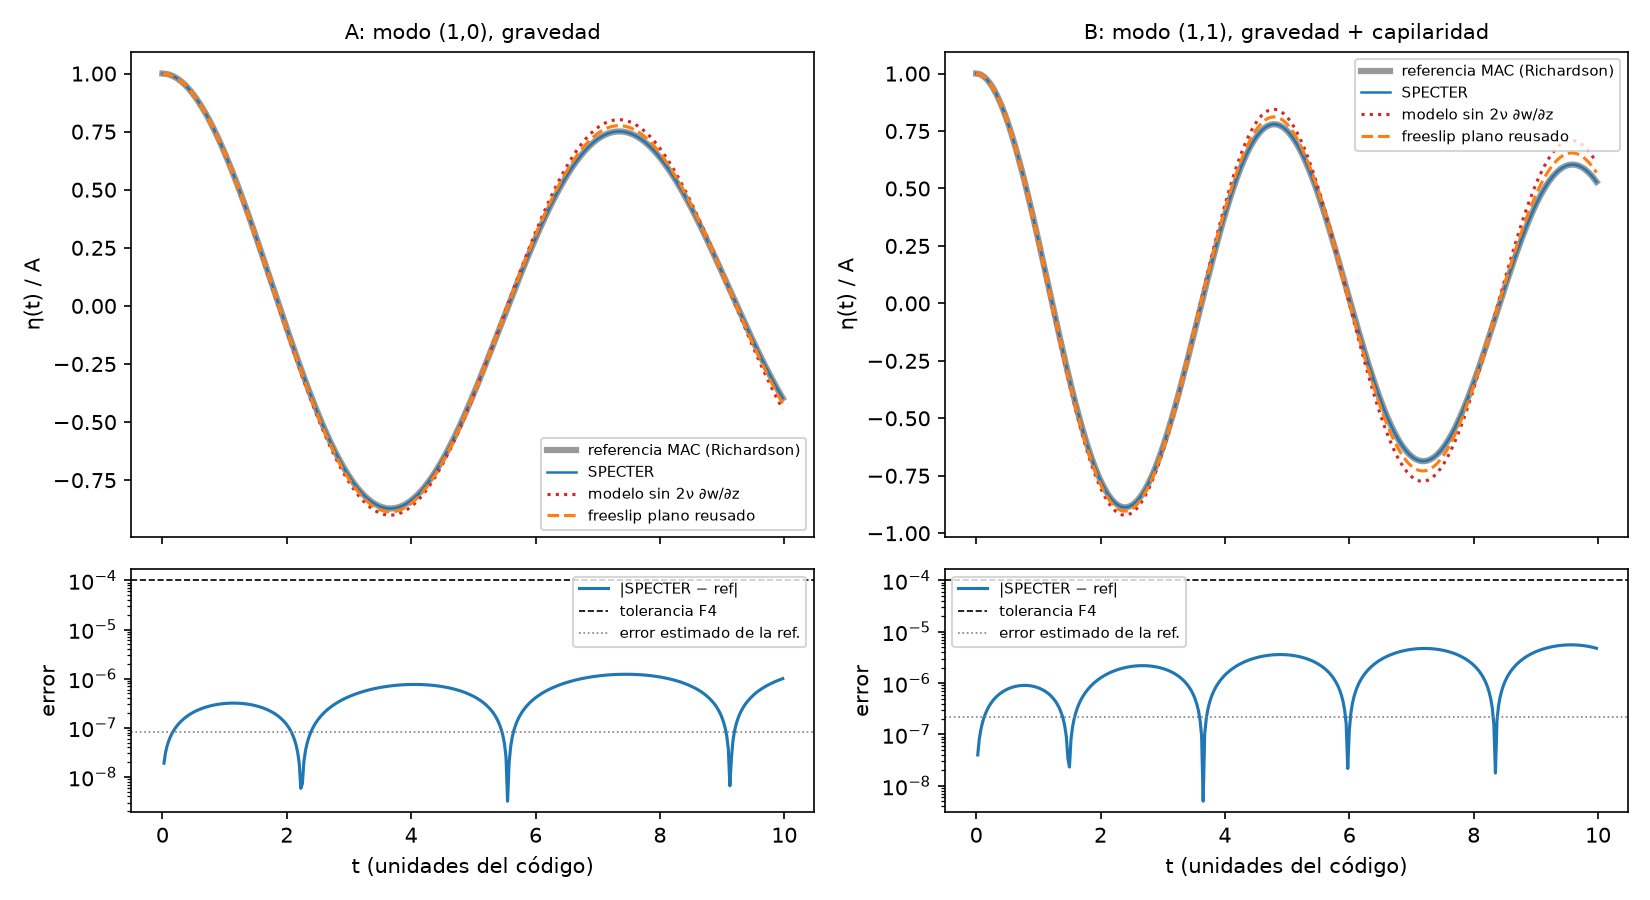
\includegraphics[width=\textwidth]{f_sd1_trayectorias.png}
\caption{Arriba: $\eta(t)/A$ de SPECTER (azul) sobre la referencia MAC (gris), y dos de los
modelos equivocados de F8 como escala de lo que la comparación detecta. Abajo: el error, con
la tolerancia de F4 y el error estimado de la referencia.}
\end{figure}

\begin{figure}[h]
\centering
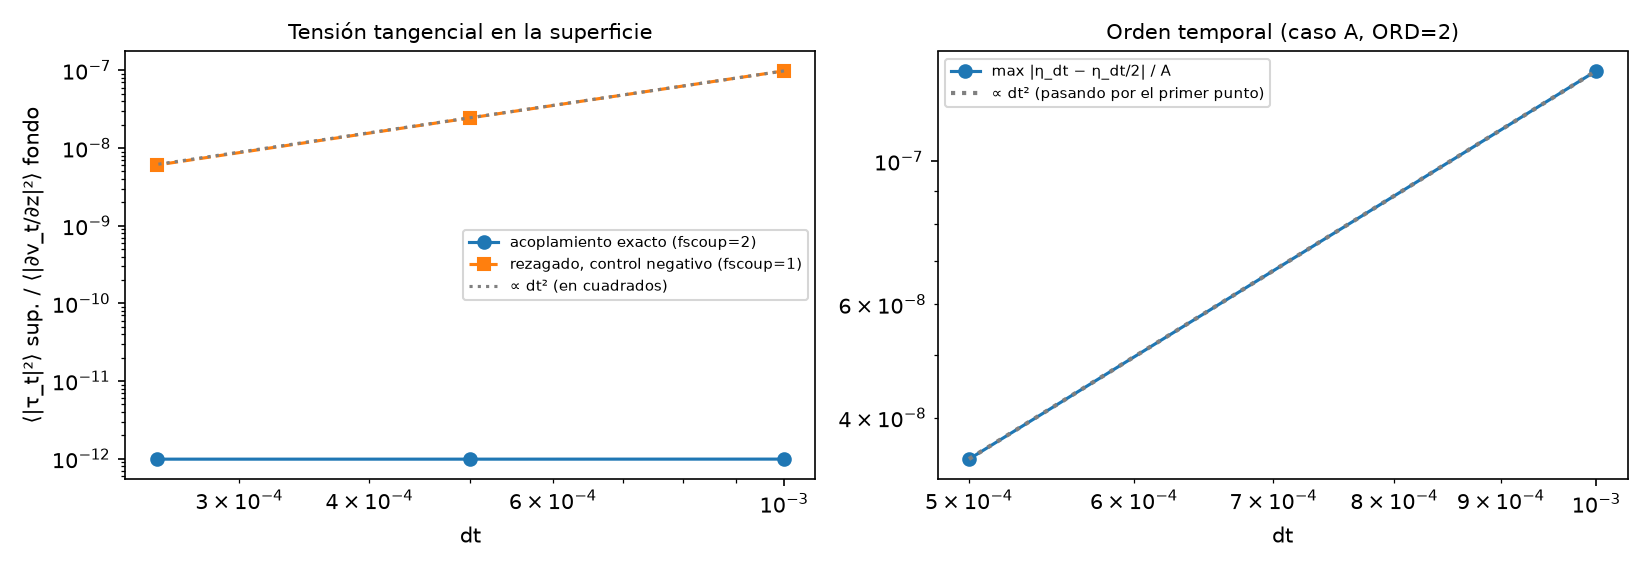
\includegraphics[width=\textwidth]{f_sd2_tension_y_orden.png}
\caption{Izquierda: tensión tangencial completa en la superficie relativa a la de la pared;
con el acople exacto queda en el nivel de reconstrucción y no depende de $dt$; con el rezagado
escala como $dt^2$ en cuadrados. Derecha: orden temporal del caso A.}
\end{figure}


\subsection{Chequeos adicionales}
\label{sec:extras}

Tres chequeos pensados después de congelar la puerta, que por eso no están en ella. Corren en
\archivo{numerico/fase5/corridas_superficie_deformable.py} (10\,min, 173\,MB), que guarda
además las series de las figuras en
\archivo{salidas/tablas/superficie_deformable_corridas.json} (copia en
\archivo{verificacion/logs/fase5_extras_2026-09-28.json}).

\begin{description}
\item[E1, desacople toroidal (§\ref{sec:toroidal}).] Un modo
  $v_y=u_0\sin(\pi z/2L_z)\cos x$, con $w=0$, corrido con \texttt{freesurface} y con
  \texttt{freeslip}: las dos energías coinciden \textbf{exactamente} (diferencia relativa
  máxima $0{,}0$), la tasa es $3{,}467401099\cdot10^{-2}$ contra $3{,}467401100\cdot10^{-2}$ de
  la referencia de diferencias finitas de la Fase~2 más $\nu k^2$ ($4{,}2\cdot10^{-10}$), y
  $\eta$ queda idénticamente en cero. El desacople no es sólo del modelo: el código lo
  respeta bit a bit.
\item[E2, reinicio.] 2000 pasos, escritura de los binarios (incluido
  \archivo{fs_eta.0002.dat}), reinicio con \texttt{stat=2} y otros 2000 pasos, contra 4000
  pasos seguidos: $\eta$ coincide en los 39 tiempos comunes con una diferencia máxima de
  $1{,}9\cdot10^{-11}\,A$. No es bit a bit porque los campos se guardan en el espacio físico
  y al releerlos se recalcula su continuación FC-Gram; es del orden del redondeo de esa
  vuelta.
\item[E3, amplitud.] Desvío máximo de $\eta(t)/A$ respecto de la referencia \emph{lineal},
  caso A hasta $t=4$: $7{,}6\cdot10^{-7}$ con $A=10^{-6}$ y con $A=10^{-4}$ (el piso numérico,
  independiente de $A$), $4{,}6\cdot10^{-7}$ con $A=10^{-3}$, y $3{,}0\cdot10^{-5}$ con
  $A=10^{-2}$. A amplitud chica el término no lineal del volumen no se ve, y a
  $A=10^{-2}$ domina. Es lo esperable si, como se estima acá\propio, el modo fundamental
  recibe la primera corrección no lineal a tercer orden (relativa $\propto A^2$): pasar de
  $10^{-3}$ a $10^{-2}$ la multiplica por $\sim100$ por encima del piso.
\end{description}

\paragraph{La tensión, con tres pasos de tiempo.} En la misma corrida, el cociente de
cuadrados medios entre la tensión tangencial completa en la superficie y la de la pared es
$9{,}88$, $9{,}86$ y $9{,}86\cdot10^{-13}$ para $dt=10^{-3}$, $5\cdot10^{-4}$ y
$2{,}5\cdot10^{-4}$ con el acople exacto, y $9{,}8\cdot10^{-8}$, $2{,}4\cdot10^{-8}$ y
$6{,}0\cdot10^{-9}$ con el rezagado (exactamente $\times4$ por cada mitad de $dt$). La
discordancia entre el $W$ impuesto y el obtenido es $\sim5\cdot10^{-16}$ con el exacto y
$2{,}5$\,\% por $dt/10^{-3}$ con el rezagado.


\subsection{Regresión de la Fase 2}
\label{sec:regresion}

Se volvió a correr, sin cambios y sobre el árbol modificado, la puerta de la Fase~2,
\archivo{verificacion/test_aceptacion_fase2.py} (hash \texttt{6f0b4da4}\ldots):
\textbf{6/6}, con los mismos números que en \etq{V-09}. Residuo de tensión
$6{,}14\cdot10^{-12}$ con razón en $dt$ $1{,}00$ en las dos caras; $\lambda_0$ con error
$5{,}8\cdot10^{-10}$; cociente canal/libre $4{,}000000015$ (log
\archivo{verificacion/logs/fase2_regresion_2026-09-28.log}, 6\,min, 173\,MB). En esa corrida los caminos \texttt{noslip} y \texttt{freeslip} no
habían cambiado. Después se corrigió \texttt{freeslip\_z} \etq{D-50} y las dos puertas se
volvieron a correr: Fase~2 \textbf{6/6}, con los mismos números (V3 pasa de $1{,}061$ a
$1{,}062\cdot10^{-7}$: era ciega al defecto), y Fase~5 \textbf{8/8}
(\archivo{verificacion/logs/fase2_freeslip_corregido_2026-09-28.log},
\archivo{fase5_freeslip_corregido_2026-09-28.log}).


\subsection{Revisión independiente}

Una vez convencida la implementación, se la pasó a un revisor independiente con el rol
\emph{verifier} de \archivo{agent-team/roles/verifier.md}: escepticismo por defecto,
reproducir cada afirmación con una derivación o un cálculo propio, e intentar romperla. Tenía
prohibido correr SPECTER (por la memoria de la laptop) y trabajó leyendo el código y los logs,
con cálculos chicos en Python. Su informe completo, con el bloque de afirmaciones, está en
\archivo{verificacion/logs/verificador_fase5_2026-09-28.md}.

\paragraph{Lo que verificó por su cuenta.}
\begin{itemize}
\item el modelo \eqref{eq:modelo}, releyendo Wang--Tice--Kim en el original y resolviendo el
  DOI;
\item que \texttt{pr} guarda $(dt/o)p$;
\item que el esquema de (a)--(b) es exactamente el Runge--Kutta de SPECTER aplicado al
  sistema proyectado, porque la parte armónica de la presión es una fuerza explícita en el
  rango de la proyección;
\item la condición \eqref{eq:tension} y sus signos arriba y abajo;
\item la exactitud del acople en dos pasadas: la cadena es lineal y diagonal por modo, y entre
  pasadas no se lee \texttt{pr};
\item los coeficientes de la rama nueva de \texttt{laplace\_z}, incluido $k=0$, y
  \texttt{sol\_project\_fs};
\item el desacople toroidal, también en el esquema discreto;
\item la referencia de la puerta, por tres caminos. Con $\nu\to0$ reproduce la frecuencia
  inviscida a $5\cdot10^{-10}$ (la fórmula analítica, que él sí podía usar). Con viscosidad
  coincide a $10^{-8}$ con un problema de autovalores en Chebyshev que escribió él. La
  trayectoria $\eta(t)$ coincide con su expansión modal a $\le2\cdot10^{-7}$;
\item el balance de energía y sus pesos;
\item los números de F1--F8 y de E1--E3. Además comparó SPECTER contra su propia referencia:
  $1{,}2\cdot10^{-6}$ y $5{,}4\cdot10^{-6}$;
\item el álgebra de estabilidad;
\item \textbf{el mecanismo del defecto de §\ref{sec:defecto}}, en un modelo de juguete con
  las tablas FC-Gram reales. Sólo la proyección no cambia nada. La vuelta de $u$ sola (el
  camino \texttt{noslip}) decae a $4\cdot10^{-13}$. La vuelta de $u$ y $w$ (el camino
  \texttt{freeslip}) deja un cambio fijo por subpaso, que no decae. En la energía de los
  puntos físicos es $-1{,}24\cdot10^{-8}$ con $N_z=128$ y $-2{,}2\cdot10^{-7}$ con $N_z=64$:
  el mismo signo y el mismo orden que midió SPECTER.
\end{itemize}

\paragraph{Lo que refutó o dejó abierto, y qué se hizo.}
\begin{itemize}
\item \emph{Que el efecto de la deformación sobre $\alpha$ se pueda medir con esta
  implementación.} A $O(\mathrm{Fr}^2)$ entran términos $\eta\,\partial_z(\cdot)$ que el
  modelo lineal descarta. Aceptado, y agregado en §\ref{sec:toroidal}, §\ref{sec:celda} y
  \etq{H-21}.
\item \emph{Que el amortiguamiento $2\nu k^2$ de la estimación de estabilidad sea
  conservador.} Es falso para $kh\gtrsim3$, por 2--4\,\%, aunque la cota de $dt$ vale igual.
  Corregido en el texto y en el script.
\item \emph{Un comentario del código} que llamaba exacta a
  $\partial_zw=-i(k_xv_x+k_yv_y)$: vale a precisión FC. Corregido.
\item \emph{Las cifras de F4 del pedido de revisión} eran las de la primera corrida. En este
  informe figuran las de la segunda.
\item \emph{Que la energía de \archivo{balance.txt} sea la del dominio extendido}, como
  decía la primera versión de §\ref{sec:defecto}. Es la de los puntos físicos
  (\texttt{energy()} suma \texttt{k = 1,nz-Cz}), y se comprobó leyendo la rutina. Por lo
  tanto el defecto del camino \texttt{freeslip} plano \emph{es} disipación espuria física.
  Corregido. El comentario de la puerta de la Fase~2 que atribuía a eso un factor de
  normalización entre $\langle v^2\rangle$ y $\langle\omega^2\rangle$ también estaba
  equivocado en la causa, que es \etq{H-22}; la puerta no se editó.
\item \emph{Cuánto sesga las tasas de la Fase~4}: sin decidir, depende del $dt$ y del $v_z$
  de esas corridas (§\ref{sec:defecto}).
\end{itemize}

\paragraph{Errores de código que encontró, corregidos.}
\begin{itemize}
\item Con $k_{x0}=0$ y $k_{y0}$ en Nyquist, la inicialización de $\eta$ escribía dos veces el
  mismo coeficiente. Ahora esos modos se rechazan.
\item El rms de $\eta$ contaba dos veces la columna de Nyquist en $k_x$.
\item Una variable calculada y no usada.
\end{itemize}
Después de corregirlos, las dos puertas se volvieron a correr: \PuertaFinal{} y
\FaseDosRegresion.

\paragraph{Lo que encontró fuera del alcance.} \textbf{Un error de upstream}
\etq{H-22}. En \archivo{src/pseudo/pseudospec_hd.f90}, la enstrofía de
\archivo{balance.txt} llama dos veces a \texttt{curlk(a,c,C1,2)} y nunca a
\texttt{curlk(a,b,C1,3)}: omite $\omega_z$ y cuenta $\omega_y$ dos veces. Se comprobó leyendo
el código. Es la causa de la discrepancia que \etq{H-17} había registrado sin encontrarla, y
por la que el proyecto ya había dejado de usar esa columna. No afecta a las puertas, que
comparan tasas de modos con $\omega_z=0$.

\paragraph{Un chequeo que pidió.} E1 usaba un modo toroidal con $k_y=0$, un caso débil. Se
agregó E1b, con el modo oblicuo $\mathbf k=(1,1)$:
$\mathbf v=u_0\sin(\pi z/2L_z)\cos(x+y)\,(1,-1)/\sqrt2$, que ejercita las dos
componentes tangenciales. \texttt{freesurface} y \texttt{freeslip} vuelven a dar energías
idénticas (diferencia $0{,}0$); la tasa es $4{,}467401098\cdot10^{-2}$ contra
$\nu[(\pi/2)^2+2]=4{,}467401100\cdot10^{-2}$ ($3{,}3\cdot10^{-10}$), y $\eta\equiv0$
(\archivo{verificacion/logs/fase5_e1b_toroidal_oblicuo_2026-09-28.json}).


%=====================================================================
\section{Qué implica para la celda}
\label{sec:celda}

Las cuentas son de \archivo{numerico/fase5/superficie_deformable_escalas.py}, con $h$, $\nu$,
el $k$ del forzado y el campo del PIV de \archivo{codigo/celda.py}, y $g$, $\rho$, $\sigma$ de
agua limpia declarados en \archivo{numerico/fase4/superficie_libre_escalas.py} (no son del
electrolito; supuesto de \etq{D-28}). La parte poloidal se calcula con la misma referencia
MAC de la puerta, importada, en variables adimensionales y con Richardson (error relativo
$\lesssim10^{-5}$).

\begin{figure}[h]
\centering
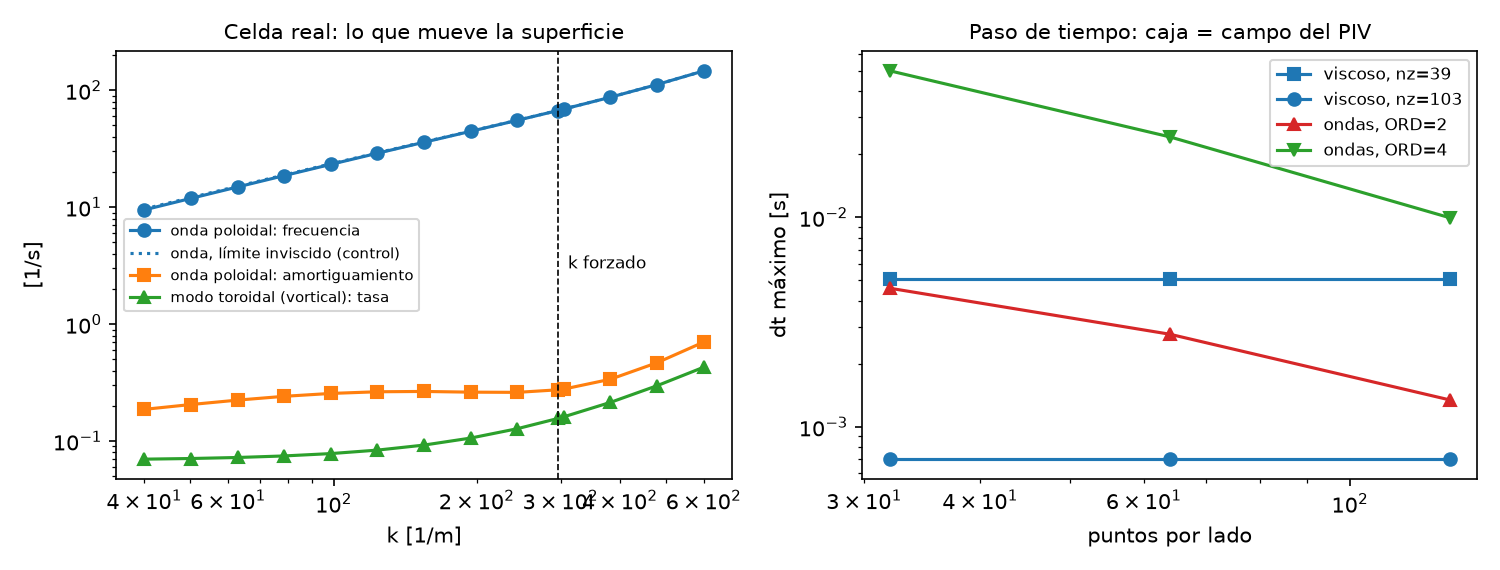
\includegraphics[width=\textwidth]{superficie_deformable_escalas.png}
\caption{Izquierda: en la celda real, la parte poloidal de cada modo es una onda de
gravedad-capilaridad (frecuencia y amortiguamiento), y la parte toroidal ---el flujo
vortical--- decae con $\lambda=\nu[(\pi/2h)^2+k^2]$ sin sentir la deformación
(§\ref{sec:toroidal}). La línea punteada es el límite inviscido, como control: la
frecuencia viscosa queda apenas por debajo, por la capa límite de fondo. Derecha: paso de
tiempo máximo con la caja igual al campo del PIV.}
\label{fig:celda}
\end{figure}

\paragraph{Lo que mueve la superficie.} En el $k$ del forzado ($296\,\mathrm{m^{-1}}$) la onda
tiene $\omega=67\,\mathrm{s^{-1}}$ (período $0{,}09$\,s) y se amortigua a
$0{,}28\,\mathrm{s^{-1}}$, contra $0{,}156\,\mathrm{s^{-1}}=2{,}28\,\alpha$ del modo
toroidal. Como la parte toroidal no siente la deformación (§\ref{sec:toroidal}), \textbf{la
superficie deformable no cambia $\alpha$ a orden lineal, exactamente}. Su efecto es no
lineal: la presión dinámica levanta la superficie $\eta\sim U^2/g$, y una estimación de orden
de magnitud\propio{} del efecto relativo es $\mathrm{Fr}^2\sim10^{-4}$ (con
$\mathrm{Fr}\sim10^{-2}$ de \etq{D-28}), no medida. Para \etq{P-02} esto descarta la
deformación lineal como explicación del déficit. Medir la no lineal completa no se puede con
esta implementación (§\ref{sec:toroidal}): pide el orden cuadrático en la frontera.

\paragraph{Lo que cuesta.} Las ondas se integran en forma explícita\propio. Con
\texttt{ORD=2} el Runge--Kutta no tiene intervalo de estabilidad sobre el eje imaginario,
$|G|^2=1+(\omega\,dt)^4/4$, y la estabilización viene sólo del amortiguamiento viscoso de la
onda; tomándolo como $2\nu k^2$ (el de superficie) sale
$dt<(16\nu k^2/\omega^4)^{1/3}$ en el $k$ máximo retenido (regla de 2/3, supuesta). Con
\texttt{ORD=4}, $dt\le2\sqrt2/\omega$. El verificador mostró que para $kh\gtrsim3$ el
amortiguamiento real es 2--4\,\% \emph{menor} que $2\nu k^2$, así que llamarlo conservador
habría sido falso; aun así, con el autovalor exacto el límite RK2 da $2{,}83$ y
$1{,}36\cdot10^{-3}$\,s contra $2{,}77$ y $1{,}35\cdot10^{-3}$\,s de la fórmula en $64^2$ y
$128^2$: la cota vale. Contra el límite viscoso vertical
$dt\le2/(\nu(\pi/\Delta z)^2)$:

\begin{center}\small
\begin{tabular}{rrcccc}
\toprule
malla & $N_z$ físico & $dt$ viscoso [s] & ondas, ORD=2 [s] & ondas, ORD=4 [s] & viscoso / ondas ORD=2\\
\midrule
$32^2$ & 39 & $5{,}1\cdot10^{-3}$ & $4{,}6\cdot10^{-3}$ & $5{,}0\cdot10^{-2}$ & 1{,}1\\
$64^2$ & 39 & $5{,}1\cdot10^{-3}$ & $2{,}8\cdot10^{-3}$ & $2{,}4\cdot10^{-2}$ & 1{,}8\\
$128^2$ & 39 & $5{,}1\cdot10^{-3}$ & $1{,}3\cdot10^{-3}$ & $1{,}0\cdot10^{-2}$ & 3{,}8\\
$64^2$ & 103 & $7{,}0\cdot10^{-4}$ & $2{,}8\cdot10^{-3}$ & $2{,}4\cdot10^{-2}$ & 0{,}25\\
\bottomrule
\end{tabular}
\end{center}

Con la malla vertical de las corridas de la Fase~4 ($N_z=64$, 39 puntos físicos) y
\texttt{ORD=2}, las ondas bajan el paso admisible entre $1{,}1$ y $3{,}8$ veces según la
malla horizontal; con \texttt{ORD=4} no limitan. Es una estimación de estabilidad lineal, no
validada con bibliografía ni con corridas a esa resolución, y el \texttt{ORD=4} no se probó
con la puerta. Elegir el orden y el paso de producción es una decisión, no una optimización
mecánica.


%=====================================================================
\section{Lo que falta y las decisiones abiertas}
\label{sec:falta}

\paragraph{Decisiones que quedan para Lucía.}
\begin{itemize}
\item \emph{Resuelta:} \etq{P-03}, el camino \texttt{freeslip} plano. Corregido y medido
  (\etq{D-50}, §\ref{sec:defecto}).
\item \textbf{Orden y paso de tiempo si se usa la superficie deformable en producción}
  (§\ref{sec:celda}). No hace falta para $\alpha$ a orden lineal.
\end{itemize}

\paragraph{Lo que el modelo no hace.}
\begin{itemize}
\item \textbf{La geometría no lineal de la superficie.} El modelo es lineal en la frontera:
  la jerarquía cúbica de la sesión anterior
  (\archivo{research/2026-09-25_nonlinear_free_surface/}) es el paso siguiente natural,
  porque resuelve este mismo operador lineal una vez por orden, con los términos de orden
  superior como dato. Más allá de pocos órdenes hace falta una coordenada que siga la
  superficie (ALE), con operadores de coeficientes variables en todo el volumen: es un
  proyecto de otra escala. Un grafo tampoco representa olas que rompen.
\item \textbf{Validación a resolución de producción.} La puerta usa $8\times8\times128$; la
  estabilidad con capilaridad en $k$ grande, \texttt{ORD=4}, y más de dos procesos MPI no se
  probaron.
\item \textbf{Reinicio.} $\eta$ se escribe y se relee (\archivo{fs_eta.NNNN.dat}); E2 lo
  prueba (§\ref{sec:extras}). La primera corrida de un reinicio recalcula $B_{\mathbf k}$ y
  las trazas a partir del campo leído.
\end{itemize}

\paragraph{Problemas encontrados en el camino.}
\begin{itemize}
\item La referencia de Chebyshev de cuarto orden empeoraba al refinar y se reemplazó por la
  MAC de segundo orden con Richardson.
\item Un chequeo del límite de tapa rígida ($g\to\infty$ contra \texttt{freeslip}) se
  descartó antes de congelar la puerta: arrancando con $\eta=0$ se excitan ondas cuyo efecto
  escala como $g^{-1/2}$ y no como $g^{-1}$, así que el criterio habría sido frágil. Se
  reemplazó por F7, que es exacto.
\item El aborto de SPECTER upstream ante una cadena desconocida termina en un
  \emph{segmentation fault}, probablemente porque llama
  \texttt{MPI\_FINALIZE(MPI\_COMM\_WORLD, ierr)}, con un argumento de más (inferencia, no
  verificada). La puerta de la Fase~2 lo acepta porque sólo pide que aborte. No se tocó; el
  código nuevo aborta con \texttt{MPI\_ABORT}.
\item La hipótesis de la condición inicial incompatible como causa del F6 fallido era
  razonable y resultó falsa; se refutó con la referencia antes de tocar código.
\item La primera corrección del defecto (reconstruir sólo el incremento del subpaso) no
  cambió nada y se sacó del código.
\end{itemize}


%=====================================================================
\begin{thebibliography}{9}
\bibitem{fontana2020} M.~Fontana, O.~P.~Bruno, P.~D.~Mininni y P.~Dmitruk,
  \emph{Fourier continuation method for incompressible fluids with boundaries},
  Comput.\ Phys.\ Commun.\ \textbf{256}, 107482 (2020).
  DOI \href{https://doi.org/10.1016/j.cpc.2020.107482}{10.1016/j.cpc.2020.107482};
  arXiv:2002.01392. Leído en el original, §§4.1--4.4 (verificado contra Crossref el
  2026-09-07, \archivo{bibliografia/REFERENCIAS.md}).
\bibitem{wtk2014} Y.~Wang, I.~Tice y C.~Kim, \emph{The viscous surface-internal wave
  problem: global well-posedness and decay}, Arch.\ Rational Mech.\ Anal.\ \textbf{212},
  1--92 (2014). DOI
  \href{https://doi.org/10.1007/s00205-013-0700-2}{10.1007/s00205-013-0700-2};
  arXiv:1109.1798. Leído en el original, §1.1, ecs.\ (1.3)--(1.8) (verificado contra
  Crossref el 2026-09-28). Se usa sólo la superficie superior; sus teoremas no se usan.
\end{thebibliography}

\end{document}
